%% ma: L12-B13-0031
%% lop: 12
%% chuong: 4
%% bai: 13
%% dang: 12.13.2
%% loai: TLN
%% muc: VD
%% dap_an: "144"
%% nguon: "(NBV)-ĐỀ SỐ 14-MỖI NGÀY 1 ĐỀ THI 2025.pdf (D14, MỖI NGÀY 1 ĐỀ - Đề số 14), Phần III Câu 6"
%% kien_thuc: "Bài 13 (thể tích vật thể qua diện tích thiết diện)"
%% trang_thai: chinh-thuc
%% ghi_chu: "Đáp án gốc đúng (144 = 16r^3/3). Hình dựng lại bằng phép chiếu song song (hai khối trụ cắt vuông góc), mang tính minh họa."
\begin{ex}
Cho hai khối trụ có bán kính đáy bằng $3$ và có trục là hai đường thẳng cắt nhau và vuông góc với nhau (xem hình vẽ). Gọi $(H)$ là phần giao nhau của hai khối trụ đó. Tính thể tích của $(H)$.
\begin{center}
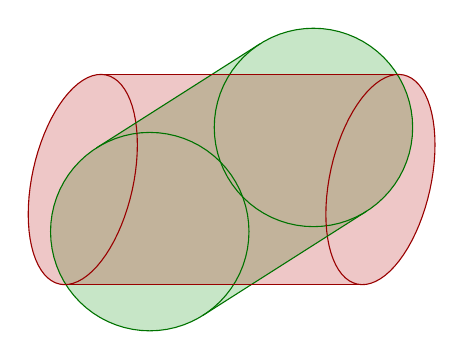
\begin{tikzpicture}[scale=.42,line join=round]
\fill[green!55!black,fill opacity=.22] (-5.475,-1.575) -- (-5.471,-1.732) -- (-5.459,-1.889) -- (-5.438,-2.044) -- (-5.409,-2.199) -- (-5.373,-2.351) -- (-5.328,-2.502) -- (-5.276,-2.650) -- (-5.216,-2.795) -- (-5.148,-2.937) -- (-5.073,-3.075) -- (-4.991,-3.209) -- (-4.902,-3.338) -- (-4.806,-3.463) -- (-4.704,-3.582) -- (-4.596,-3.696) -- (-4.482,-3.804) -- (-4.363,-3.906) -- (-4.238,-4.002) -- (-4.109,-4.091) -- (-3.975,-4.173) -- (-3.837,-4.248) -- (-3.695,-4.316) -- (-3.550,-4.376) -- (-3.402,-4.428) -- (-3.251,-4.473) -- (-3.099,-4.509) -- (-2.944,-4.538) -- (-2.789,-4.559) -- (-2.632,-4.571) -- (-2.475,-4.575) -- (-2.318,-4.571) -- (-2.161,-4.559) -- (-2.006,-4.538) -- (-1.851,-4.509) -- (-1.699,-4.473) -- (-1.548,-4.428) -- (-1.400,-4.376) -- (-1.255,-4.316) -- (-1.113,-4.248) -- (-0.975,-4.173) -- (-0.841,-4.091) -- (4.109,-0.941) -- (4.238,-0.852) -- (4.363,-0.756) -- (4.482,-0.654) -- (4.596,-0.546) -- (4.704,-0.432) -- (4.806,-0.313) -- (4.902,-0.188) -- (4.991,-0.059) -- (5.073,0.075) -- (5.148,0.213) -- (5.216,0.355) -- (5.276,0.500) -- (5.328,0.648) -- (5.373,0.799) -- (5.409,0.951) -- (5.438,1.106) -- (5.459,1.261) -- (5.471,1.418) -- (5.475,1.575) -- (5.471,1.732) -- (5.459,1.889) -- (5.438,2.044) -- (5.409,2.199) -- (5.373,2.351) -- (5.328,2.502) -- (5.276,2.650) -- (5.216,2.795) -- (5.148,2.937) -- (5.073,3.075) -- (4.991,3.209) -- (4.902,3.338) -- (4.806,3.463) -- (4.704,3.582) -- (4.596,3.696) -- (4.482,3.804) -- (4.363,3.906) -- (4.238,4.002) -- (4.109,4.091) -- (3.975,4.173) -- (3.837,4.248) -- (3.695,4.316) -- (3.550,4.376) -- (3.402,4.428) -- (3.251,4.473) -- (3.099,4.509) -- (2.944,4.538) -- (2.789,4.559) -- (2.632,4.571) -- (2.475,4.575) -- (2.318,4.571) -- (2.161,4.559) -- (2.006,4.538) -- (1.851,4.509) -- (1.699,4.473) -- (1.548,4.428) -- (1.400,4.376) -- (1.255,4.316) -- (1.113,4.248) -- (0.975,4.173) -- (0.841,4.091) -- (-4.109,0.941) -- (-4.238,0.852) -- (-4.363,0.756) -- (-4.482,0.654) -- (-4.596,0.546) -- (-4.704,0.432) -- (-4.806,0.313) -- (-4.902,0.188) -- (-4.991,0.059) -- (-5.073,-0.075) -- (-5.148,-0.213) -- (-5.216,-0.355) -- (-5.276,-0.500) -- (-5.328,-0.648) -- (-5.373,-0.799) -- (-5.409,-0.951) -- (-5.438,-1.106) -- (-5.459,-1.261) -- (-5.471,-1.418) -- cycle;
\fill[red!70!black,fill opacity=.22] (-6.150,-1.050) -- (-6.148,-1.206) -- (-6.141,-1.358) -- (-6.130,-1.506) -- (-6.114,-1.651) -- (-6.094,-1.791) -- (-6.069,-1.926) -- (-6.040,-2.055) -- (-6.007,-2.179) -- (-5.970,-2.298) -- (-5.929,-2.409) -- (-5.884,-2.515) -- (-5.835,-2.613) -- (-5.782,-2.704) -- (-5.726,-2.788) -- (-5.667,-2.864) -- (-5.604,-2.932) -- (-5.538,-2.992) -- (-5.470,-3.044) -- (-5.399,-3.088) -- (-5.325,-3.123) -- (-5.249,-3.150) -- (-5.171,-3.168) -- (-5.091,-3.177) -- (-5.010,-3.178) -- (3.990,-3.178) -- (4.073,-3.170) -- (4.157,-3.153) -- (4.242,-3.127) -- (4.328,-3.093) -- (4.414,-3.051) -- (4.500,-3.000) -- (4.586,-2.941) -- (4.672,-2.874) -- (4.758,-2.799) -- (4.843,-2.716) -- (4.927,-2.626) -- (5.010,-2.529) -- (5.091,-2.424) -- (5.171,-2.314) -- (5.249,-2.196) -- (5.325,-2.073) -- (5.399,-1.944) -- (5.470,-1.810) -- (5.538,-1.671) -- (5.604,-1.527) -- (5.667,-1.379) -- (5.726,-1.227) -- (5.782,-1.072) -- (5.835,-0.914) -- (5.884,-0.753) -- (5.929,-0.591) -- (5.970,-0.426) -- (6.007,-0.261) -- (6.040,-0.095) -- (6.069,0.072) -- (6.094,0.238) -- (6.114,0.403) -- (6.130,0.568) -- (6.141,0.731) -- (6.148,0.892) -- (6.150,1.050) -- (6.148,1.206) -- (6.141,1.358) -- (6.130,1.506) -- (6.114,1.651) -- (6.094,1.791) -- (6.069,1.926) -- (6.040,2.055) -- (6.007,2.179) -- (5.970,2.298) -- (5.929,2.409) -- (5.884,2.515) -- (5.835,2.613) -- (5.782,2.704) -- (5.726,2.788) -- (5.667,2.864) -- (5.604,2.932) -- (5.538,2.992) -- (5.470,3.044) -- (5.399,3.088) -- (5.325,3.123) -- (5.249,3.150) -- (5.171,3.168) -- (5.091,3.177) -- (5.010,3.178) -- (-3.990,3.178) -- (-4.073,3.170) -- (-4.157,3.153) -- (-4.242,3.127) -- (-4.328,3.093) -- (-4.414,3.051) -- (-4.500,3.000) -- (-4.586,2.941) -- (-4.672,2.874) -- (-4.758,2.799) -- (-4.843,2.716) -- (-4.927,2.626) -- (-5.010,2.529) -- (-5.091,2.424) -- (-5.171,2.314) -- (-5.249,2.196) -- (-5.325,2.073) -- (-5.399,1.944) -- (-5.470,1.810) -- (-5.538,1.671) -- (-5.604,1.527) -- (-5.667,1.379) -- (-5.726,1.227) -- (-5.782,1.072) -- (-5.835,0.914) -- (-5.884,0.753) -- (-5.929,0.591) -- (-5.970,0.426) -- (-6.007,0.261) -- (-6.040,0.095) -- (-6.069,-0.072) -- (-6.094,-0.238) -- (-6.114,-0.403) -- (-6.130,-0.568) -- (-6.141,-0.731) -- (-6.148,-0.892) -- cycle;
\draw[green!45!black,domain=0:360,samples=73] plot ({3*cos(\x)+-2.475},{3*sin(\x)+-1.575});
\draw[green!45!black,domain=0:360,samples=73] plot ({3*cos(\x)+2.475},{3*sin(\x)+1.575});
\draw[red!60!black,domain=0:360,samples=73] plot ({-4.500+1.650*cos(\x)},{3*sin(\x)+1.050*cos(\x)});
\draw[red!60!black,domain=0:360,samples=73] plot ({4.500+1.650*cos(\x)},{3*sin(\x)+1.050*cos(\x)});
\draw[green!45!black] (-4.086,0.956)--(0.864,4.106);
\draw[green!45!black] (-0.864,-4.106)--(4.086,-0.956);
\draw[red!60!black] (-3.955,3.178)--(5.045,3.178);
\draw[red!60!black] (-5.045,-3.178)--(3.955,-3.178);
\end{tikzpicture}
\end{center}
\shortans{144}
\loigiai{Chọn hệ tọa độ $Oxyz$ với $O$ là giao điểm hai trục, trục của hai khối trụ là $Ox$ và $Oy$. Hai khối trụ là $y^2+z^2\le9$ và $x^2+z^2\le9$.
Mặt phẳng $z=t$ ($-3\le t\le3$) cắt $(H)$ theo hình vuông $|x|\le\sqrt{9-t^2}$, $|y|\le\sqrt{9-t^2}$ có cạnh $2\sqrt{9-t^2}$, diện tích $S(t)=4(9-t^2)$.
$V=\displaystyle\int_{-3}^{3}4(9-t^2)\,\mathrm dt=4\Big(54-18\Big)=144$.}
\end{ex}
